\documentclass[a4paper]{article}
\usepackage{amsfonts}
\usepackage{amsmath}
\usepackage{amssymb}
\usepackage{graphicx}
\usepackage{float}

\begin{document}
  
\noindent \large Auteur: Siebe Mees \\
\noindent \large Studierichting: Informatica\\
\noindent \large Oefeningenreeks 5G nr. 6.5\\

\medskip

\normalsize

Gegeven: $f(x)=2x-x^2$ en $g(x)=x$\\

\begin{enumerate}

\item Snijpunten\\

$2x - x^2 = x$\\

$x - x^2 = 0$\\

$x(1 - x) = 0$\\

$x = 0 $ en $ x = 1$\\

\item Bovenste functie bepalen\\

$x = \dfrac{1}{2}$\\

$\left \{
\begin{array}{l}
f\left(\dfrac{1}{2}\right) = 2 \cdot \dfrac{1}{2} - \left(\dfrac{1}{2}\right)^2 = \dfrac{3}{4} \\

g\left(\dfrac{1}{2}\right) = \dfrac{1}{2} \\

\end{array}
\right .$\\

$ \Rightarrow f $ boven $ g$\\

\item Volume\\

$V = \pi \displaystyle\int_0^1 \left((2x - x^2)^2 - x^2 \right) dx$\\

$= \pi \displaystyle\int_0^1 (4x^2 - 4x^3 + x^4 - x^2) dx$\\

$= \pi \displaystyle\int_0^1 (3x^2 - 4x^3 + x^4) dx$\\

$= \pi \left[ \dfrac{3x^3}{3} - \dfrac{4x^4}{4} + \dfrac{x^5}{5} \right]_0^1$\\

$= \pi \left[ x^3 - x^4 + \dfrac{x^5}{5} \right]_0^1$\\

$= \pi \left( \left(1 - 1 + \dfrac{1}{5}\right) - (0 - 0 + 0) \right)$\\

$= \dfrac{\pi}{5}$\\

\end{enumerate}

\begin{tabular}{c|ccccc}
$x$ & $0$ & & $1$ & & $2$ \\ \hline
$f(x)$ & $0$ &  & $+$ &  & $0$ \\
$f'(x)$ & $+$ & & $0$ & & $-$ \\
$f''(x)$ & $-$ & & $-$ & & $-$ \\ \hline
$f(x)$ & $0$ & $\nearrow$ & $M(1)$ & $\searrow$ & $2$ \\
 &  & $\frown$ &  & $\frown$ & \\
\end{tabular}\\

\begin{tabular}{c|cc}
$x$ & $0$ & \\ \hline
$g(x)$ & $0$ & $+$ \\
$g'(x)$ & $+$ & \\ \hline
$g(x)$ & $0$ & $\nearrow$ \\
\end{tabular}\\

\begin{figure}[H]
\centering
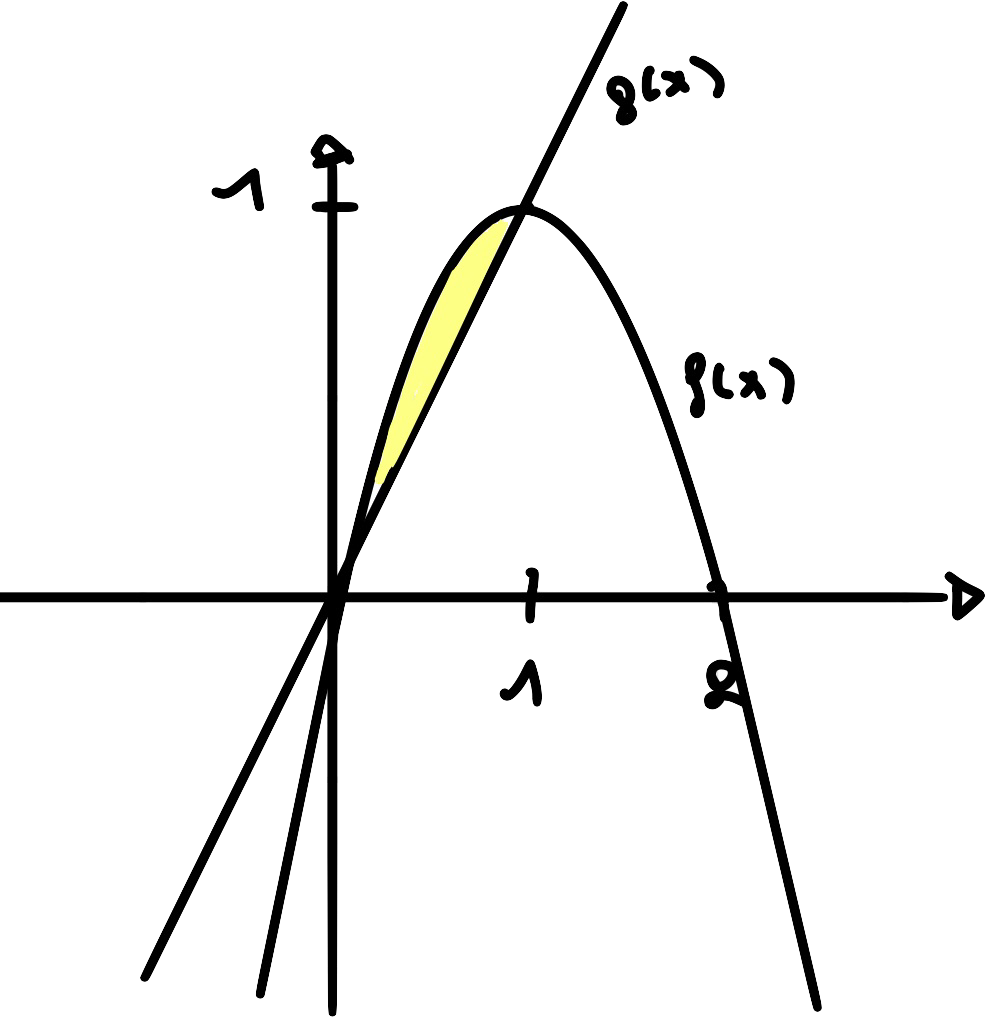
\includegraphics[width=5cm]{5G-6.5-siebe.mees.INF.png}
\end{figure}

\begin{thebibliography}{999}
%\bibitem{a} Referentie
\end{thebibliography}
\end{document} 
